\chapter{Schiere di antenne}

	Vedremo in questo capitolo come combinare in modo opportuno una serie di antenne per migliorare le prestazioni del nostro ricevitore.

\section{Schiera di antenne isotrope}
	Il primo caso che analizzeremo è quello di una serie lineare ed equispaziata di antenne isotrope, ovvero antenne che irradiano in modo uniforme in tutte le direzioni.

	Questa semplificazione permette di considerare le proprietà del posizionamento delle antenne nell'\emph{array} astraendo dalle caratteristiche specifiche delle varie antenne.

	\begin{figure}[ht]
		\centering
		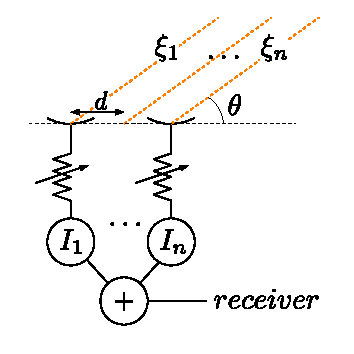
\includegraphics{img/schiera_antenne.pdf}
		\caption{Le antenne della schiera sono alimentate dalle correnti $I_i$ e ricevono il segnale dal campo lontano con sfasamenti diversi $\xi_i$.}
		\label{fig:schiera}
	\end{figure}

	Dallo schema elettrico in figura \ref{fig:schiera} si può facilmente calcolare il segnale in arrivo al ricevitore, definito come \gls{af}.

	\begin{esp} \label{eq:array_factor}
		AF = \sum_{i=1}^n I_i e^{\jmath \xi_i}
			\stackrel{(*)}{=} \sum_{i=1}^n I_i ~ e^{\jmath (i-1) \beta d \cos \theta}
	\end{esp}
	dove in (*) si calcola la differenza di cammino tra i vari percorsi.

	\subsection{Schiere fasate}
		Un caso particolare, ma di notevole interesse, sono le \emph{schiere fasate}, array in cui le correnti hanno modulo uguale e sfasamento $\alpha$.
		Il calcolo dell'\gls{af} per questa scelta dei parametri si semplifica ulteriormente.

		\begin{esp}
				AF
				& = \sum_{k=0}^{n-1} I_k ~ e^{\jmath k \beta d \cos \theta} \\
				& \stackrel{(1)}{=}  \sum_{k=0}^{n-1} A_k ~ e^{\jmath k (\beta d \cos \theta + \alpha)}
					\stackrel{(2)}{=} \sum_{k=0}^{n-1} ~ A_k e^{\jmath k \psi} \\
				& = A_o \sum_{k=0}^{n-1} e^{\jmath k \psi}
					\stackrel{(3)}{=} A_o
						\left( \frac{ 1 - e^{\jmath n \psi} }{ 1 - e^{\jmath \psi} } \right) \\
				& = A_o
						~ \frac{ e^{\jmath \frac{n}{2} \psi} }{ e^{\jmath \psi} }
						\left( \frac{ e^{\jmath \frac{n}{2} \psi} - e^{- \jmath \frac{n}{2} \psi} }{ e^{\jmath \psi} - e^{-\jmath \psi} } \right) \\
				& = A_o
					\left( \frac{ \sin(\frac{n}{2} \psi) }{ \sin(\frac{\psi}{2}) } \right)
					~ e^{\jmath \frac{n-1}{2} \psi}
			\end{esp}
		dove
		\begin{itemize}
			\item[(1)] $I_k$ viene scomposto in modulo e fase come $A_k ~ e^{\jmath k \alpha}$
			\item[(2)] l'angolo $\psi$ è definito, per semplificare la notazione, come lo sfasamento complessivo tra un'antenna e la successiva
			\item[(3)] viene utilizzata la formula per il calcolo della serie geometrica troncata.
		\end{itemize}

		\subsubsection{Regione di visibilità}
			I valori validi di $\theta$, ovvero l'inclinazione dell'onda incidente rispetto all'array, sono nell'intervallo $[0, \pi]$: le proprietà dell'array per i valori opposti sono ottenute semplicemente per simmetria.

			Questo induce dei limiti nell'angolo $\psi$: il range di valori validi per questo angolo è detto \emph{regione di visibilità}.
			\begin{equation} \begin{gathered}
			0 \le \theta \le \pi \\
			-\beta d \le \beta d \cos \theta \le \beta d \\
			\alpha - \beta d \le \psi \le \alpha + \beta d
			\end{gathered} \end{equation}

		\subsubsection{Massimo di radiazione}
			Il massimo delle capacità dell'antenna si ha per $\psi = 0$, che corrisponde all'angolo (o agli angoli) $\theta_0$ nella regione di visibilità per cui $\beta d \cos \theta_0 = -\alpha$.

			\begin{esp}
				|AF(\psi = 0)|
					& = A_0
						~ \left( \lim_{\psi \to 0} \frac{ \sin(\frac{n}{2} \psi) }{ \sin(\frac{\psi}{2}) } \right)
						~ \left| e^{\jmath \frac{n-1}{2} \psi} \right|
						= A_0 \cdot n \cdot 1 = A_0 \cdot n
			\end{esp}

			Questa osservazione ci permette di calcolare il pattern di radiazione dell'array, definito come il modulo dell'\gls{af} normalizzato al suo valor massimo.

			\begin{equation} \label{eq:array_pattern}
				F(\theta)
					= \frac{1}{n} \, \frac{\sin(\frac{n}{2} \psi) }{ \sin( \frac{\psi}{2} ) }
					= \frac{1}{n} \, \frac{
						\sin \left(
							\frac{n}{2} (\beta d \cos \theta + \alpha)
						\right)
					}{
						\sin \left(
							\frac{(\beta d \cos \theta + \alpha)}{2}
						\right)
					}
			\end{equation}

		\subsubsection{Minimo di radiazione}
			Osservando l'equazione \eqref{eq:array_pattern} si può notare che gli zeri del campo lontano si hanno per valori di $\psi$ che annullano il numeratore, ma non il denominatore.

			\begin{esp}
				\frac{1}{n} \, \frac{\sin(\frac{n}{2} \psi) }{ \sin( \frac{\psi}{2} ) } = 0
				\Leftrightarrow
					\frac{n}{2} \psi = \pm m \pi \quad \forall m \neq 0
			\end{esp}

		\subsubsection{Lobi secondari}
			Lobi secondari troppo pronunciati possono minare la direttività dell'array, per questo motivo è utile calcolarne l'entità.

			Cerco quindi i massimi della funzione \gls{af}.

			\begin{esp}
				\deriv{AF}{\psi}
				& = \deriv{}{\psi} \left(
						\frac
							{ \sin(\frac{n}{2} \psi) }
							{ \sin( \frac{\psi}{2} ) }
					\right) \\
				& = \frac{1}{\sin^2 \left(\frac{\psi}{2}\right)} \left[
					\cos \left(\frac{n}{2} \psi \right) \frac{n}{2} \sin\left( \frac{\psi}{2} \right)
					- \sin \left(\frac{n}{2} \psi \right) \cos\left( \frac{\psi}{2} \right)
					\right]
				 = 0
			\end{esp}

			Per valori di $n$ grandi (indicativamente maggiori di 10), si può compiere questa semplificazione.

			\begin{esp}
				\cos \left(\frac{n}{2} \psi \right) \sin\left( \frac{\psi}{2} \right)
				= \frac{2}{n} \sin \left(\frac{n}{2} \psi \right) \cos\left( \frac{\psi}{2} \right)
				\simeq 0 \quad \forall n \to +\infty
			\end{esp}

			Le soluzioni dell'equazione precedente sono quindi
			\begin{equation*}
				\begin{dcases}
					\psi = 0, \, \pi
						& \text{non accettabili, perché punti di massimo} \\
					\psi = \pm \frac{\pi}{n} \, (2p + 1) \quad \forall p \in \mathbb{N}
						& \text{validi se rientrano nella regione di visibilità}
				\end{dcases}
			\end{equation*}

			Ottenute le posizioni di massimi e minimi in $\psi$ è possibile calcolare attraverso la funzione $AF(\psi)$ il valore di \gls{sll}, misura del rapporto tra lobi primari e secondari.
			Assumendo che esista il primo lobo secondario, otteniamo che $\psi_1 = \frac{3\pi}{n}$. Il valore assoluto dell'array factor per il primo lobo secondario, quindi, risulta pari a
			\begin{equation}
				|AF(\psi_1) | = \left|\frac{sin\left(\pm n \frac{3 \pi}{2 n}\right)}{sin\left(\pm \frac{3\pi}{2 n}\right)}\right| \approx \frac{2n}{3\pi}
			\end{equation}
Poiché nel lobo principale l'array factor è $|AF(\psi=0)|=n$, il side lobe level risulta indipendente dal numero di antenne della schiera ed è pari a

\begin{equation}
	SLL=10\,log_{10}\left|\frac{AF(\psi_1)}{AF(\psi=0)}\right|^2 = 20\,log_{10}\left(\frac{2}{3\pi}\right) \approx -13,5dB
\end{equation}
	\subsection{Tipologie di schiere lineari fasate}
		Come si può notare dalla definizione di $\psi$, il massimo che si ha per $\psi = 0$ corrisponde ad un valore di $\theta$ che è funzione dello sfasamento delle correnti $\alpha$.

		La possibilità di spostare il lobo principale in modo elettronico, senza quindi variazioni meccaniche della schiera, è un punto di forza di questa tipologia di antenne perché le rende riconfigurabili ``al volo''.

		A seconda dei valori di $\alpha$, le schiere lineari fasate si dividono in
		\begin{esp*}
			\alpha = 0
			& \implies \theta_0 = \frac{\pi}{2}
			& \text{schiere \emph{broadside}} \\
			\alpha = \pm \beta d
			& \implies \theta_0 = 0 \land \theta_0 = \pi
			& \text{schiere \emph{endfire}} \\
		\end{esp*}
\clearpage
\section{Larghezza del lobo al primo zero}
Vogliamo ora identificare l'angolo all'interno del quale si estende il massimo di radiazione della schiera, \textbf{BWFN} \emph{Beam Width at First Null}. Divideremo l'analisi nel caso la schiera sia un broadside o un endfire array.

\subsubsection{Broadside array: $\alpha=0$}
Nel caso broadside, i primi due minimi si trovano risolvendo
\begin{esp}
	\frac{n}{2}\beta d & cos(\theta_{FN}) = \pm \pi \quad \Leftrightarrow \quad \frac{n \pi}{\lambda} \, d \, cos(\theta_{FN})=\pm 1\\
	\theta_{FN_{1/2}}&= cos^{-1}\left(\pm\frac{\lambda}{n d}\right)
\end{esp}
Il BWFN sarà quindi
\begin{esp}
	BWFN &= \left| \theta_{FN_{left}} - \theta_{FN_{right}}\right| =  \left|cos^{-1}\left(-\frac{\lambda}{n d}\right) - cos^{-1}\left(\frac{\lambda}{n d}\right) \right| \\
	&\stackrel{n d\, \gg\, \lambda}{\approx} \left| \frac{\pi}{2}- \frac{\lambda}{n d} -\left(\frac{\pi}{2} + \frac{\lambda}{n d}\right)\right|\\
	BWFN &\approx \frac{2\lambda}{n d}
\end{esp}

\subsubsection{Endfire array: $\alpha=\pm \beta d$}
Nel caso broadside, i primi due minimi si trovano risolvendo

\begin{esp*}
	\frac{n}{2}\beta d &\left[ cos(\theta_{FN})\pm 1\right] = \pm \pi \quad \Leftrightarrow \quad \frac{n \pi}{\lambda} \, d \, \left[ cos(\theta_{FN})\pm 1\right]=\pm 1
\end{esp*}
\begin{equation*} cos(\theta_{FN}) =
	\begin{cases}
		\frac{\lambda}{n \, d} - 1 & \text{Le altre possibilità non danno}\\
		-\frac{\lambda}{n \, d} + 1 & \text{un valido }\theta_{FN}~ (cos(\theta)\in [-1;1])
	\end{cases}
\end{equation*}


Utilizzando le formule di duplicazione del coseno:


\begin{equation}
	cos(x)=cos^2\left(\frac{x}{2}\right)-sin^2\left(\frac{x}{2}\right) = 2 cos^2\left(\frac{x}{2}\right)-1 = 1 - 2 sin^2\left(\frac{x}{2}\right)
\end{equation}

\clearpage
possiamo riscrivere le due soluzioni come
\begin{enumerate}
	\item \begin{esp}
	&cos(\theta_{FN}) = \frac{\lambda}{n \, d} - 1 \Leftrightarrow cos(\theta_{FN}) +1 = \frac{\lambda}{n \, d} \\
	& \Leftrightarrow  2 cos^2\left(\frac{\theta_{FN}}{2}\right) = \frac{\lambda}{n \, d}\\
	&\implies \theta_{FN} = 2 arcos\left(\pm \sqrt{\frac{\lambda}{2n \, d}}\right)
\end{esp}
che per $n d \gg \lambda$
\begin{equation*}
	\theta_{FN_{1/2}} \approx \pi \mp 2 \sqrt{\frac{\lambda}{2n \, d}}
\end{equation*}

\item
\begin{esp}
&cos(\theta_{FN}) = -\frac{\lambda}{n \, d} + 1 \Leftrightarrow 1 - cos(\theta_{FN})  = \frac{\lambda}{n \, d} \\
& \Leftrightarrow  2 sin^2\left(\frac{\theta_{FN}}{2}\right) = \frac{\lambda}{n \, d}\\
&\implies \theta_{FN} = 2 arcsin\left(\pm \sqrt{\frac{\lambda}{2n \, d}}\right)
\end{esp}
che per $n d \gg \lambda$
\begin{equation*}
\theta_{FN_{1/2}} \approx \pm 2 \sqrt{\frac{\lambda}{2n \, d}}
\end{equation*}
\end{enumerate}

In entrambi i casi la soluzione porta a
\begin{esp}
	BWFN &= \left| \theta_{FN_{left}} - \theta_{FN_{right}}\right| \approx 4\frac{\lambda}{2 n \, d}
\end{esp}
\section{Schiera di antenne non isotrope}
	Osserveremo ora il caso generico in cui le antenne isotrope ideali sono rimpiazzate da antenne reali.

	\subsection{Schiera di dipoli corti}
		\begin{figure}[ht]
			\centering
			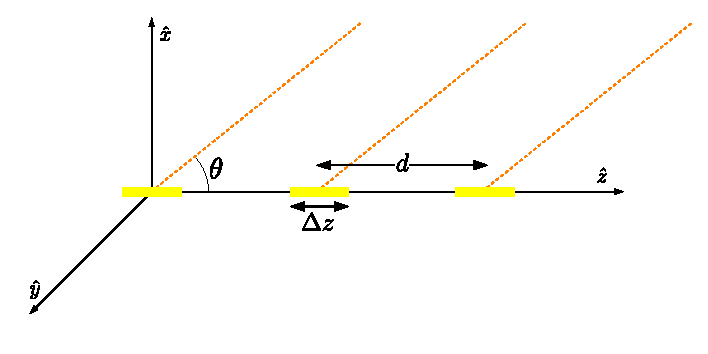
\includegraphics{img/schiera_non_isotropa_dipoli_corti.pdf}
			\caption{I dipoli corti di lunghezza $\Delta z$ sono equispaziati da una distanza $d$.}
			\label{fig:schiera_non_isotropa_dipoli_corti}
		\end{figure}

		In figura \ref{fig:schiera_non_isotropa_dipoli_corti} i dipoli corti sono disposti lungo l'asse $z$: il contributo nel potenziale vettore magnetico dell'antenna $k$-esima si può valutare, nel campo lontano, come segue.

		\begin{esp}
			\vec{A}_k(\r)
				& = \frac{\mu}{4\pi}
				\left( \frac{e^{-\jmath \beta (r - k d \cos \theta)}}{r - k d \cos \theta} \right)
				I_k \Delta z \, \hat{z} \\
				& \simeq \frac{\mu}{4\pi}
				\left( \frac{e^{-\jmath \beta (r - k d \cos \theta)}}{r} \right)
				I_k \Delta z \, \hat{z}
		\end{esp}
		dove il termine di sfasamento al denominatore dell'onda sferica è trascurabile perché nel campo lontano $d \ll r$. Il termine all'esponenziale invece non lo è, perché nel caso generale $d$ è paragonabile alla lunghezza d'onda $\lambda$.

		L'effetto complessivo delle $n$ antenne si può quantificare come
		\begin{esp}
			\vec{A}(\r)
			& = \sum_{k=0}^{n-1} \vec{A}_k(\r) \\
			& = \frac{\mu}{4\pi}
				\left( \frac{e^{-\jmath \beta r}}{r} \right)
				\Delta z
				\left( \sum_{k=0}^{n-1} I_k ~ e^{\jmath k \beta d \cos \theta} \right) \hat{z} \\
			& = \frac{\mu}{4\pi}
				\left( \frac{e^{-\jmath \beta r}}{r} \right)
				\Delta z ~ AF \, \hat{z}
		\end{esp}
		dove l'\gls{af} è calcolato come il rapporto tra il contributo complessivo e quello della singola antenna.

		Il campo elettrico, per esempio lungo $\theta$, si può ricavare a partire da $\vec{A}$.
		\begin{esp}
			\vec{E}_\theta
			& = \left[
					\jmath \frac{\eta_0}{2\lambda}
					\left( \frac{e^{-\jmath \beta r}}{r} \right)
					\Delta z \, \sin \theta \, \hat{z}
				\right] AF
		\end{esp}
		dove il termine tra tra quadre è il campo lontano della singola antenna.

	\subsection{Schiera di antenne filiformi generiche}
		Abbiamo osservato nella precedente sezione come il campo della singola antenna si componga nella schiera con l'\gls{af}, definito in precedenza per le antenne isotrope.

		Questa calcolo si può generalizzare per distribuzioni lineari di corrente $i_k(z)$ generiche.

		\begin{figure}[ht]
			\centering
			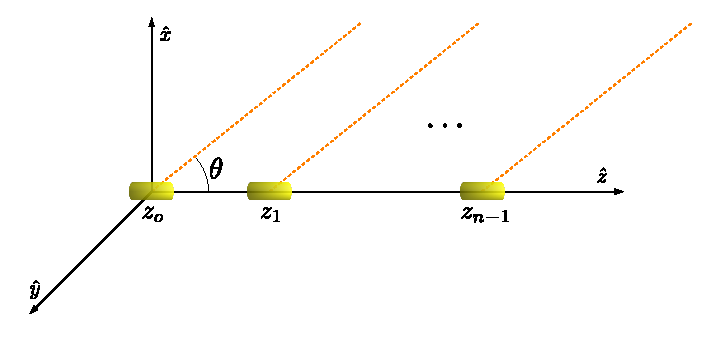
\includegraphics{img/schiera_non_isotropa_dipoli.pdf}
			\caption{I dipoli sono posti nei punti $z_0, \ldots, z_{n-1}$.}
			\label{fig:schiera_non_isotropa_dipoli}
		\end{figure}

		Il potenziale vettore magnetico nel campo lontano si calcola come
		\begin{esp}
			\vec{A}_k(\r)
				& \stackrel{(1)}{=} \frac{\mu}{4\pi}
				\left( \frac{e^{-\jmath \beta r}}{r} \right)
				\int_{V_s} \vec{J}(\r^{\, \prime})
					~ e^{\jmath \beta r^\prime \cos \theta} \de \r^{\, \prime} \\
				& \stackrel{(2)}{=} \frac{\mu}{4\pi}
				\left( \frac{e^{-\jmath \beta r}}{r} \right) \hat{z}
				\int_{-\infty}^{+\infty}
					\left( \sum_{k=0}^{n-1} i_k(z^\prime) ~ e^{\jmath \beta z^\prime \cos \theta} \right)
					\de z^\prime
		\end{esp}
		dove
		\begin{itemize}
			\item[(1)] il termine esponenziale è scomposto in ciò che dipende da $\r$, posizione del punto in esame rispetto all'origine, e da $\r^{\,\prime}$, posizione del punto rispetto alla sorgente infinitesima di corrente $\vec{J}$
			\item[(2)] la corrente è rivolta solamente lungo l'asse $z$, quindi il prodotto tra vettori si riduce ad un prodotto tra scalari.
		\end{itemize}

		Da $\vec{A}$ si può ricavare $E_\theta$, come fatto in precedenza.
		\begin{esp} \label{eq:e_theta_schiera_dipoli}
			\vec{E}_\theta
			& = \jmath \frac{\eta_0}{2\lambda}
					\left( \frac{e^{-\jmath \beta r}}{r} \right)
					\sum_{k=0}^{n-1}
						\int_{-\infty}^{+\infty}  ~ i_k(z^\prime) \, e^{\jmath \beta z^\prime \cos \theta} ~dz^\prime \, \hat{z} \\
			& = \jmath \frac{\eta_0}{2\lambda}
					\left( \frac{e^{-\jmath \beta r}}{r} \right)
					\sum_{k=0}^{n-1} E_k(\theta) \\
		\end{esp}
		dove il termine integrale $E_k(\theta)$ è identificabile come il contributo della $k$-esima antenna della schiera.

	\subsection{Schiera di antenne filiformi identiche}
		Nel caso specifico in cui tutte le antenne abbiano la stessa lunghezza $L$ e la stessa distribuzione di corrente, è possibile scomporre ancora scomporre il campo nel constributo della tipologia di antenna e di array.

		Prima di tutto, definiamo la distribuzione di correnti complessiva delle $n$ antenne.
		\begin{esp}
			i_n(z^\prime) = I_n ~ i(z^\prime - z_n)
		\end{esp}
		dove $i(\cdot)$ è una funzione reale (quindi un numero puro) ed associa alla distanza dal centro dell'antenna $n$-esima la frazione di corrente presente rispetto a $I_n$.

		Il contributo dell'antenna nel campo lontano si può valutare con la seguente espressione.
		\begin{esp}
			E_n(\theta)
			& = \sin \theta ~ I_n
				\, \int_{z_n - \frac{L}{2}}^{z_n + \frac{L}{2}} \,
					i(z^\prime - z_n) e^{\jmath \beta z^\prime \cos \theta}~ dz^\prime  \\
			& \stackrel{(*)}{=} \sin \theta ~ I_n
				\, \int_{-\frac{L}{2}}^{+\frac{L}{2}} \,
					i(\tau) ~ e^{\jmath \beta (\tau + z_n) \cos \theta}~d\tau  \\
			& = \sin \theta ~ I_n ~ e^{\jmath \beta z_n \cos \theta}
				\, \int_{-\frac{L}{2}}^{+\frac{L}{2}} \,
					i(\tau) ~ e^{\jmath \beta \tau \cos \theta} ~d\tau ~\\
		\end{esp}
		dove in (*) $z^\prime$ è stato sostituito da $\tau = z^\prime - z_n$.

		È possibile infine inserire questo risultato all'interno della formula generale, in equazione \eqref{eq:e_theta_schiera_dipoli}.
		\begin{esp}
			\vec{E}_\theta
			= \jmath \frac{\eta_0}{2\lambda}
					\left( \frac{e^{-\jmath \beta r}}{r} \right)
					\underbrace{
						\left( \sum_{k=0}^{n-1} I_k ~ e^{\jmath \beta z_k \cos \theta} \right)
					}_{\text{AF}}
					\underbrace{
						\left( \sin \theta \int_{-\frac{L}{2}}^{+\frac{L}{2}} \,
						i(\tau) ~ e^{\jmath \beta \tau \cos \theta}~d\tau \right)
					}_{\text{singola antenna}}
		\end{esp}
		dove sono messi in luce i contributi della singola antenna e della loro combinazione.

		Avendo provato questa proprietà per il campo elettrico, essa vale anche per il pattern di radiazione, che non è altro che il campo lontano normalizzato al suo valore massimo.
		\begin{esp}
			F(\theta, \phi) = F_{AF}(\theta, \phi) ~ F_{elemento}(\theta, \phi)
		\end{esp}

	\subsection{Schiera non uniformemente eccitate}
		In questa sezione mostreremo come il valore massimo $I_n$ di corrente nell'antenna $n$-esima si possa sfruttare per ottenere particolari effetti sul pattern di radiazione.

		Per esempio, sono interessanti le antenne che sopprimono completamente i lobi secondari, possedendo quindi un \gls{sll} pari a 0.

		Questo si può raggiungere ponendo $AF = 1 + e^{\jmath \psi}$, che corrisponde a $F_{AF} = \cos\left( \frac{\pi}{2} \cos \theta \right)$: questa condizione è in particolare verificata per $n$ antenne alimentate come descritto.

		\begin{esp}
			& (1 + e^{\jmath \psi}) \text{ non ha lobi secondari } \\
			& \implies (1 + e^{\jmath \psi})^n =
				\sum_{k=0}^{n-1} \binom{n}{k} e^{\jmath k \psi} \text{ non ha lobi secondari }
		\end{esp}

		Ponendo le correnti nel rapporto ``binomiale'' che sussiste tra i termini dell'\gls{af} è possibile quindi sopprimere completamente i lobi secondari.
%%% Local Variables:
%%% mode: latex
%%% TeX-master: "antenne"
%%% End:
